\scanpage{3}
\unsure{CF|CP} \uline{$\overline{\mathrm{VIII}}$}

% margin note written slanted, above the left branch
\margin{\uline{NB} Un magasin ``local'' \unsure{ce. qui|ce qui} \unsure{se réfère|réfère} à \deleted{\unsure{des}} \unsure{rels} \unsure{particulières} \unsure{d'incidence} aux \uline{lieux}.}

\diagram{
\begin{tikzcd}[ampersand replacement=\&,column sep=1em,row sep=2.6em,/tikz/scale=0.70,/tikz/transform shape]
\& \begin{gathered}
\text{\uline{Magasins généraux}}\\
M,\ \leq,\ \ll,\ |\circ|\\
\mathrm{Mag}\,1-\mathrm{Mag}\,4\ (\text{p.22})\\
\Sigma_M\subset\unsure{P|\mathcal P|\mathscr P}(M)
\end{gathered}\arrow[-,dl]\arrow[-,dr] \& \\
\begin{gathered}
\text{\uline{Magasins locaux}}\\
M,\ \leq,\ \overset{\circ}{\ll},\ |\circ|_{\unsure{\mathcal L|L}}\\
\mathrm{Magloc}\,1-\mathrm{Magloc}\,3\ (\text{p.23})\\
\Sigma_M\subsetP(\mathcal L)
\end{gathered}\arrow[-,dr,shift left=1.5pt]\arrow[-,dr,shift right=1.5pt]
\&\begin{gathered}(A,B\in\Sigma_M\\A\cap B=\varnothing\Longleftrightarrow A|\circ|B)\end{gathered}
\&\begin{gathered}
\text{\uline{Magasins \deleted{\unsure{transparents}}}}\\
\text{\inserted{(à Ombres) fidèles}}\\
M,\ \leq,\ \overset{\circ}{\ll}\\
\mathrm{Magfid}\,1-\mathrm{Magfid}\,2\ (\text{p.31})
\end{gathered}\arrow[-,dl]\arrow[-,d]\\
\&\begin{gathered}
\text{\uline{Magasins \deleted{ponctuels}}}\\
\text{\inserted{ponctuaires}}\\
M,\ \leq,\ \overset{\circ}{\ll}\\
\mathrm{Magponc}\,1-3\ (\text{p.24}).\\
\Sigma_M\simeqP(\mathcal L)
\end{gathered}\arrow[-,d]
\&\begin{gathered}
\text{\uline{Maquettes}}\\
M,\ \leq\\
\text{\uline{Maq}}\,1:\ \leq\ \text{rel. d'ordre}\ (\text{p.25})\\
\Sigma_M\simeqP(M)
\end{gathered}\\
\&\begin{gathered}
\text{\uline{Magasins ensemblistes}}\\
\mathcal L,\ M\subset\mathrm{Fig\acute{e}l}(\mathcal L)\\
\unsure{\mathrm{Magens}|\mathrm{Magun}}\,1,\ \mathrm{Magens}\,2\ (\text{p.9})
\end{gathered}\arrow[-,d]\&\\
\&\begin{gathered}
\text{\uline{Magasins \inserted{\uline{ensemblistes}} modérés}}\\
\mathcal L,\ M\subset\mathrm{Fig\acute{e}l}(\mathcal L)\\
\mathrm{Magens}\,1-\mathrm{Magens}\,3
\end{gathered}\&
\end{tikzcd}}

% margin note below the local-magasin node
\margin{(\unsure{cette} inclusion ne commute pas néc. à $A\cap B$ \unsure{ni|m.} (ni à $\varnothing$?), et encore moins : $\operatorname{Sup}(A,B)$}

% margin note left of the ponctuaire node; added wording is above the line
\margin{\figure{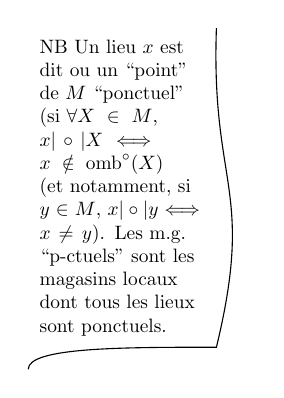
\begin{tikzpicture}[scale=0.7,transform shape]
\node[anchor=north west,align=left,text width=3cm,inner sep=0pt] (n) at (0,0) {\uline{NB} Un lieu $x$ est dit \inserted{\unsure{ou} un ``point'' de $M$} ``\uline{ponctuel}'' (\unsure{si} $\forall X\in M$, $x|\circ|X\Longleftrightarrow x\notin\mathrm{omb}^{\circ}(X)$ (et notamment, si $y\in M$, $x|\circ|y\Longleftrightarrow x\ne y$). Les \unsure{m.g.} ``\unsure{p-ctuels}'' sont les magasins locaux dont tous les lieux sont ponctuels.};
\draw ([xshift=2mm,yshift=2mm]n.north east) .. controls ([xshift=1mm]n.east) and ([xshift=9mm]n.east) .. ([xshift=2mm,yshift=-2mm]n.south east) .. controls ([yshift=-2mm]n.south) and ([xshift=-2mm,yshift=-2mm]n.south west) .. ([xshift=-2mm,yshift=-6mm]n.south west);
\end{tikzpicture}}}

% margin note to the right of the faithful-magasin branch, within a drawn enclosure
\margin{\figure{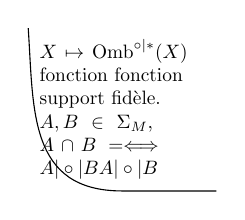
\begin{tikzpicture}[scale=0.7,transform shape]
\node[anchor=north west,align=left,text width=3cm,inner sep=0pt] (n) at (0,0) {$X\mapsto\mathrm{Omb}^{\unsure{\circ|*}}(X)$ \deleted{\unsure{fonction}} \unsure{fonction} support \uline{fidèle}. $A,B\in\Sigma_M$, $A\cap B=\varnothing\Longleftrightarrow\deleted{\unsure{A|\circ|B}}\inserted{A|\circ|B}$};
\draw ([xshift=-2mm,yshift=2mm]n.north west) .. controls ([xshift=-1mm]n.west) and ([xshift=-2mm,yshift=-2mm]n.south west) .. ([yshift=-2mm]n.south) -- ([xshift=2mm,yshift=-2mm]n.south east);
\end{tikzpicture}}}

% margin note right of Maquettes
\margin{(\uline{NB} Une maquette, \unsure{un|ou|est} espace \inserted{\unsure{ultra|ultraf.}} top. satisfaisant l'axiome de séparation $T_0$, n'est un magasin \deleted{local (avec \unsure{pour les éléments discrets|pour éléments les éléments discrets})} ponctuel que si elle est discrète.}

% margin note left of the ensembliste node
\margin{Ce \unsure{sont} les seuls magasins qui \deleted{\unsure{sont|soit}} correspondent aux \unsure{pts de vues} communément \unsure{admis} pour ``la topologie''}

% margin note left of the modere node
\margin{Correspondent à \deleted{des} ``topologies modérées'', qui n'ont été \unsure{développées} à présent que pour la seule structure linéaire par morceaux \unsure{sur} $\mathbb R$}

% margin note right of the modere node
\margin{NB Il y a des magasins modérés non ensemblistes, p. ex. les maquettes.}

\uline{NB} Je préfère finalement, dans $M$, noter $\unlhd$ la relation d'incidence, et noter de $\unsure{=|\simeq}$ la relation d'incidence entre $M$ et $F$. La notation $\triangleleft$ sera l'incidence stricte. La relation d'inclusion entre figures sera notée $\deleted{\unsure{\leq}}\subseteq$, \unsure{où n' confusion à craindre}, $\deleted{\unsure{\subseteq}}\leq$ (inclusion des figures). Je noterai $\overset{s}{\leq}$ pour les subdivisions \unsure{?}
% archive sheet number: 2
